\documentclass{article}
\usepackage{amsmath}
\usepackage{algorithm}
\usepackage[noend]{algpseudocode}
\usepackage{graphicx}
\usepackage{listings}
\usepackage[utf8]{inputenc}
\usepackage{array}
\usepackage{tabu}
\usepackage{color}
\usepackage{hyperref}
\usepackage{listings}
\usepackage{color}
 
\definecolor{codegreen}{rgb}{0,0.6,0}
\definecolor{codegray}{rgb}{0.5,0.5,0.5}
\definecolor{codepurple}{rgb}{0.58,0,0.82}
\definecolor{backcolour}{rgb}{0.95,0.95,0.92}
 
\lstdefinestyle{mystyle}{
    backgroundcolor=\color{backcolour},   
    commentstyle=\color{codegreen},
    keywordstyle=\color{magenta},
    numberstyle=\tiny\color{codegray},
    stringstyle=\color{codepurple},
    basicstyle=\footnotesize,
    breakatwhitespace=false,         
    breaklines=true,                 
    captionpos=b,                    
    keepspaces=true,                 
    numbers=left,                    
    numbersep=5pt,                  
    showspaces=false,                
    showstringspaces=false,
    showtabs=false,                  
    tabsize=2
}
 
\lstset{style=mystyle}


\hypersetup{
    colorlinks=true,
    linkcolor=blue,
    filecolor=magenta,      
    urlcolor=cyan,
    pdftitle={H20171030081 Report},
    bookmarks=true
}
 
\urlstyle{same}

\makeatletter
\def\BState{\State\hskip-\ALG@thistlm}
\makeatother
\graphicspath{ {./images/} }

\begin{document}

 
\thispagestyle{empty}
 
\tableofcontents
 
\listoffigures
 
\listoftables

\lstlistoflistings

\newpage
 
\pagenumbering{arabic}

\section{Introduction of Tools}

\paragraph{}
In this section, i will be introducing the tools ,languages and API's which will be used throughout the report.

\subsection{ELK Stack}
\paragraph{}
"ELK" is the acronym for three open source projects: Elasticsearch, Logstash, and Kibana.

\subsubsection{Elastic Search}

\paragraph{}
Elasticsearch is a search engine based on Lucene. It provides a distributed, multitenant-capable full-text search engine with an HTTP web interface and schema-free JSON documents.

\subsubsection{Logstash}

\paragraph{}
Logstash is an open source tool for collecting, parsing, and storing logs for future use.

\subsubsection{Kibana}

\paragraph{}
Kibana is an open source data visualization plugin for Elasticsearch. It provides visualization capabilities on top of the content indexed on an Elasticsearch cluster. Users can create bar, line and scatter plots, or pie charts and maps on top of large volumes of data.

\subsection{Honeypots}

\paragraph{}
In computer terminology, a honeypot is a trap set to detect, deflect or in some manner counteract attempts at unauthorized use of information systems.

\paragraph{}
In other words, A server that is configured to detect an intruder by mirroring a real production system. It appears as an ordinary server doing work, but all the data and transactions are phony. Located either in or outside the firewall, these are used to learn about an intruder’s techniques as well as determine vulnerabilities in the real system.”

\paragraph{}
Based on design criteria, honeypots can be classified as

\begin{enumerate}
\item Low-interaction honeypots
\item Medium-interaction honeypots
\item High-interaction honeypots
\end{enumerate}

\subsubsection{Low-interaction honeypots}
\paragraph{}
Low-interaction honeypots simulate only the services frequently requested by attackers. Since they consume relatively few resources, multiple virtual machines can easily be hosted on one physical system, the virtual systems have a short response time, and less code is required, reducing the complexity of the security of the virtual systems.
\paragraph{}
Low-interaction honeypots present the hacker emulated services with a limited subset of the functionality they would expect from a server, with the intent of detecting sources of unauthorized activity. For example, the HTTP service on low-interaction honeypots would only support the commands needed to identify that a known exploit is being attempted.

\subsubsection{Medium-interaction honeypots}
\paragraph{}
Medium-interaction honeypots  might more fully implement the HTTP protocol to emulate a well-known vendor’s implementation, such as Apache. However, there are no implementations of a medium-interaction honeypots and for the purposes of this paper, the definition of low-interaction honeypots captures the functionality of medium-interaction honeypots in that they only provide partial implementation of services and do not allow typical, full interaction with the system as high-interaction honeypots.

\subsubsection{High-interaction honeypots}
\paragraph{}
High-interaction honeypots imitate the activities of the real systems that host a variety of services. It let the hacker interact with the system as they would any regular operating system, with the goal of capturing the maximum amount of information on the attacker’s techniques. Any command or application an end-user would expect to be installed is available and generally, there is little to no restriction placed on what the hacker can do once he/she comprises the system.
\paragraph{}
According to recent researches in high interaction honeypot technology, by employing virtual machines, multiple honeypots can be hosted on a single physical machine. Therefore, even if the honeypot is compromised, it can be restored more quickly. Although high interaction honeypots provide more security by being difficult to detect, but it has the main drawback that it is costly to maintain.

\subsubsection{Cowrie Honeypot}
\paragraph{}
Cowrie is used for our research purposes.Cowrie is a medium interaction SSH and Telnet honeypot designed to log brute force attacks and the shell interaction performed by the attacker.
\paragraph{Interesting Features of Cowrie Honeypot}

\begin{enumerate}
\item Fake filesystem with the ability to add/remove files. A full fake filesystem resembling a Debian 5.0 installation is included.
\item Possibility of adding fake file contents so the attacker can cat files such as /etc/passwd. Only minimal file contents are included.
\item Logging in JSON format for easy processing in log management solutions.
\end{enumerate}

\subsection{VirusTotal}
\paragraph{}
VirusTotal is a website created by the Spanish security company Hispasec Sistemas. Launched in June 2004, it was acquired by Google Inc. in September 2012. The company's ownership switched in January 2018 to Chronicle, a subsidiary of Alphabet Inc. (Google's parent company).

\paragraph{}
VirusTotal aggregates many antivirus products and online scan engines to check for viruses that the user's own antivirus may have missed, or to verify against any false positives.Files up to 256 MB can be uploaded to the website or sent via email.Anti-virus software vendors can receive copies of files that were flagged by other scans but passed by their own engine, to help improve their software and, by extension, VirusTotal's own capability. 

\subsubsection{List of Anti-Virus Engines used by VirusTotal}


\begin{table}[h!]
\begin{center}

\begin{tabular}{ |c|c|c|c| } 
 \hline
 AegisLab & Agnitum & AhnLab & Anity\\
 \hline
 Aladdin & Avast & AVG  & Avira \\
 \hline
 BluePex  & Baidu  & BitDefender & Bkav  \\
 \hline
 ByteHero & Quick Heal & CMC Antivirus & CYREN \\
 \hline
 ClamAV  & Comodo & CrowdStrike & Doctor Web Ltd. \\
 \hline
 Emsisoft & Endgame & Eset Software & Fortinet \\
 \hline
 F-Prot  & F-Secure & G Data & Hacksoft \\
 \hline
 Hauri  & IKARUS & nProtect & Invincea  \\
 \hline
 Jiangmin & K7AntiVirus & Kaspersky & Kingsoft\\
 \hline
 Malwarebytes  & McAfee & Microsoft & eScan \\
 \hline
 Nano Security  & Norman & Panda & Rising \\
 \hline
  Symantec  & VIPRE & TotalDefense & TrendMicro \\
 \hline
 
 
 \hline
\end{tabular}
\caption{List of Antivirus Engines}
\end{center}
\end{table}

\subsection{Github}
\paragraph{}
GitHub (originally known as Logical Awesome LLC) is a web-based hosting service for version control using git. It is mostly used for computer code. It offers all of the distributed version control and source code management (SCM) functionality of Git as well as adding its own features. It provides access control and several collaboration features such as bug tracking, feature requests, task management, and wikis for every project.

\paragraph{}
The code which is written for this project is entirely pushed to Github where it is bug free and version safe.

\section{Installation of Tools}
\paragraph{}
In this section, we will be mentioning about the installation of various tools which will be used in the project.

\subsection{Elastic Search}

\begin{enumerate}
\item Download the Debian Installation file from the below link \\
\textit{\href{https://www.elastic.co/downloads/elasticsearch}}
\item Install it using the below command \\
\textit{{\color{blue}iotsys3@iotsys3-Precision-Tower-3420:~} dpkg -i elastic-search-6.2.0.deb}
\item Now start the service using below command \\
\textit{{\color{blue}iotsys3@iotsys3-Precision-Tower-3420:~} sudo service elasticsearch start}
\end{enumerate}

\paragraph{}
Open the link \textit{http://localhost:9200} in the browser and check for the ouput which should look like below.

\begin{figure}[H]
\centering
\caption{Elastic Search Output}
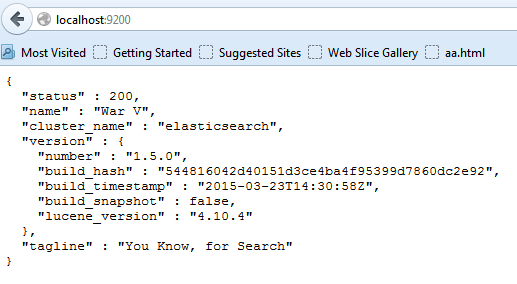
\includegraphics[scale=0.7]{Elastic_Search_Installation}
\end{figure}

\paragraph{}
We can check for the working of elastic search in the browser by typing the url \textit{http://localhost:9200} and verifying the output.

\subsection{Logstash}

\begin{enumerate}
\item Download the logstash debian installation file from below link\\
\textit{https://www.elastic.co/downloads/logstash}
\item Install it using the below command \\
\textit {{\color{blue}iotsys3@iotsys3-Precision-Tower-3420:~} dpkg -i logstash-6.2.2.deb}
\item Now start the service using below command\\
\textit{\color{blue}iotsys3@iotsys3-Precision-Tower-3420:~} sudo service logstash start
\end{enumerate}

\subsection{Kibana}

\begin{enumerate}
\item Download the Kibana debian installation file from below link\\
\textit{https://www.elastic.co/downloads/kibana}
\item Install it using the below command\\
\textit{{\color{blue}iotsys3@iotsys3-Precision-Tower-3420:~} dpkg -i kibana-6.2.2.deb}
\item Now start the service using below command\\
\textit{{\color{blue}iotsys3@iotsys3-Precision-Tower-3420:~} sudo service kibana start}
\end{enumerate}



\begin{figure}[H]
\centering
\caption{Kibana Dashboard}
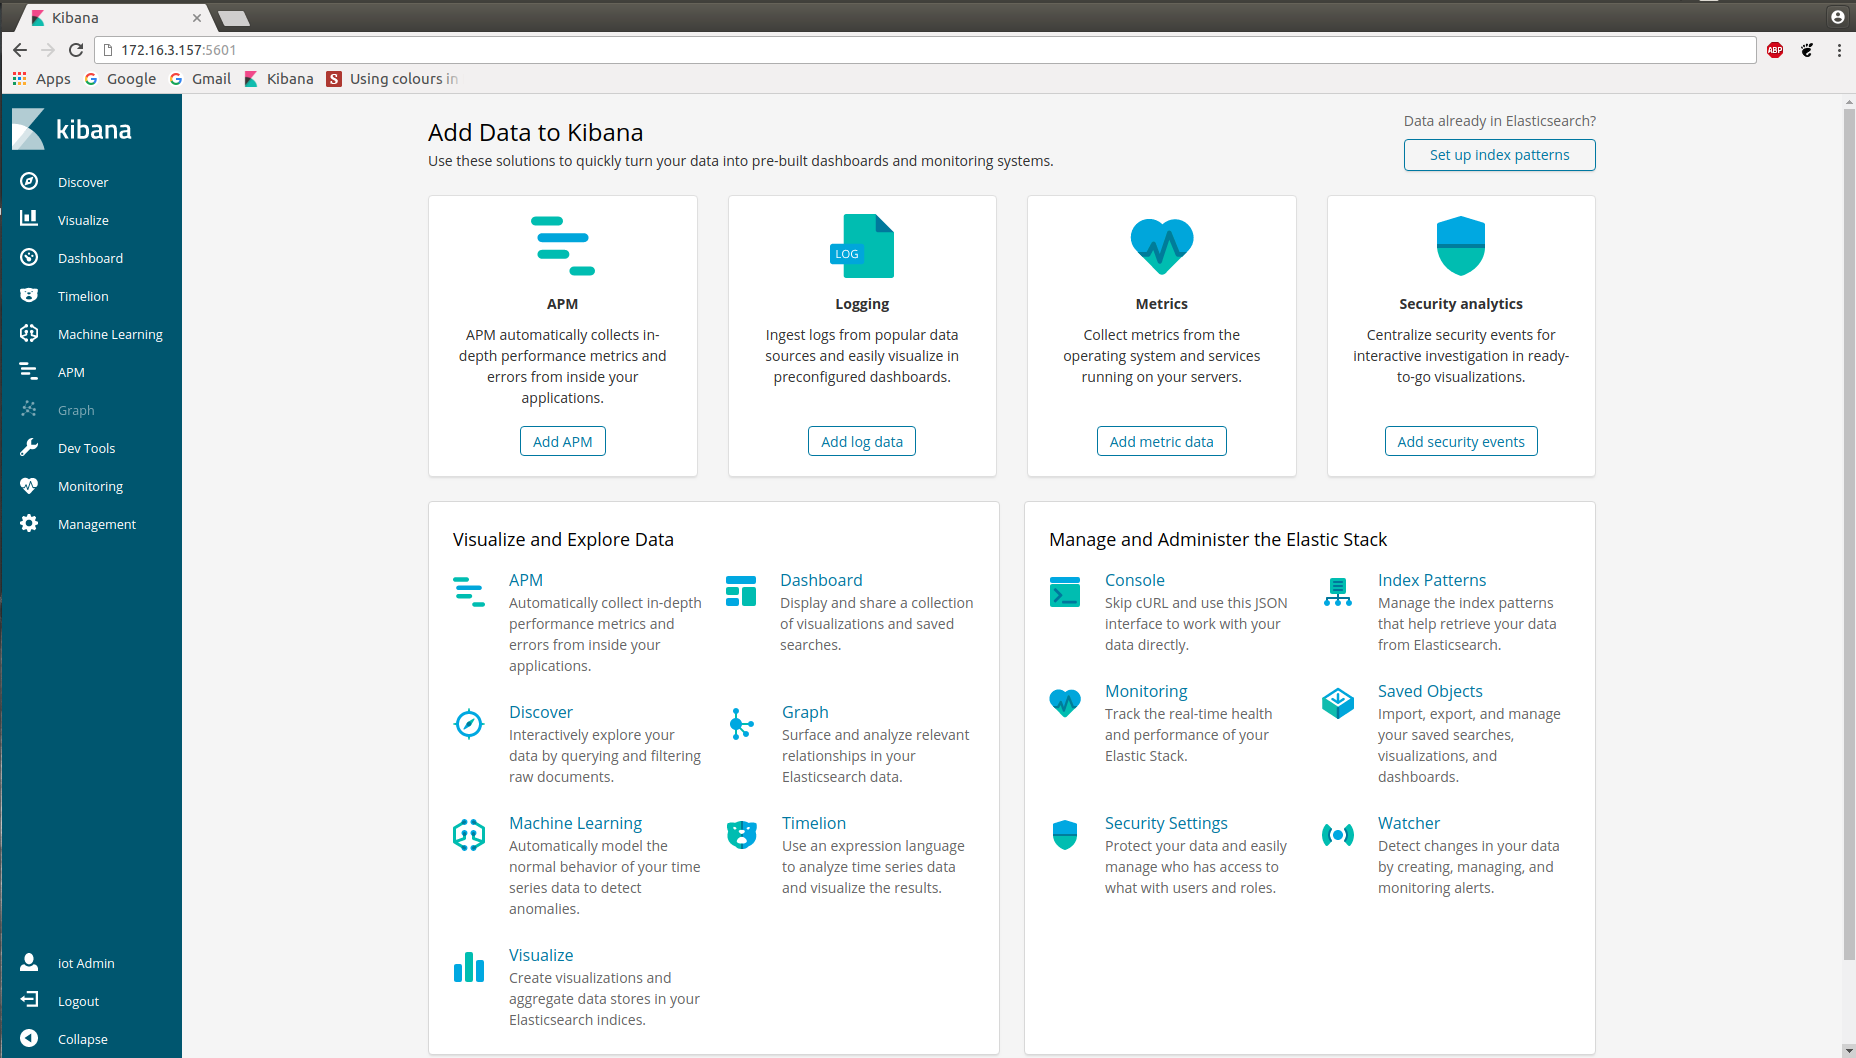
\includegraphics[scale=0.22]{Kibana_Installation}
\end{figure}

\paragraph{}
Open the link (\textit{http://localhost:5601}) in the browser and check for the Kibana Dashboard which looks like above.


\subsection{Cowrie Honeypot}

\paragraph{}
Cowrie honeypot is installed in a separate machine with public IP which is connected to the internet.It can be installed by following the steps given below.

\subsubsection{Install dependencies } 
\textit{{\color{blue}iotsys3@iotsys3-Precision-Tower-3420:} sudo apt-get install git python-virtualenv libssl-dev libffi-dev build-essential libpython-dev python2.7-minimal authbind}

\subsubsection{Create a user account } 
\textit{{\color{blue}iotsys3@iotsys3-Precision-Tower-3420:} sudo adduser --disabled-password cowrie}\\
\textit{{\color{blue}iotsys3@iotsys3-Precision-Tower-3420:} sudo su - cowrie}

\subsubsection{Checkout the code } 
\textit{{\color{blue}iotsys3@iotsys3-Precision-Tower-3420:} git clone http://github.com/micheloosterhof/cowrie}\\
\textit{{\color{blue}iotsys3@iotsys3-Precision-Tower-3420:} cd cowrie}


\subsubsection{Setup Virtual Environment } 
\textit{{\color{blue}iotsys3@iotsys3-Precision-Tower-3420:} pwd}\\
\textit{{\color{blue}iotsys3@iotsys3-Precision-Tower-3420:} virtualenv cowrie-env}

\subsubsection{Port redirection } 
\textit{{\color{blue}iotsys3@iotsys3-Precision-Tower-3420:} sudo iptables -t nat -A PREROUTING -p tcp --dport 22 -j REDIRECT --to-port 2222}

\paragraph{}
In the same folder, create a copy of \textit{cowrie.cfg.dist} and modify the file according to your needs like changing the name, SSH port number etc. 

\subsubsection{Starting Cowrie }
\textit{{\color{blue}iotsys3@iotsys3-Precision-Tower-3420:} bin/cowrie start}

\paragraph{}
Cowrie will be up and running on port 22 which will monitor all SSH logins and commands executed by the attackers or intruders.


\section{Working Model}

All the tools listed above are integrated to form a complete Working Model which looks like below.

\begin{figure}[H]
\centering
\caption{Working Model}
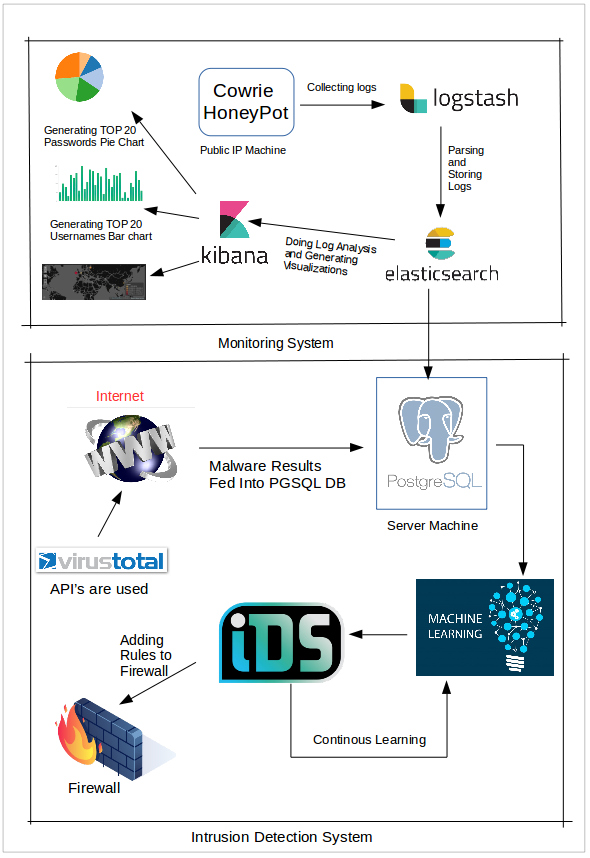
\includegraphics[scale=0.5]{Working_Model}
\end{figure}

\section{Monitoring System}
\paragraph{}
Cowrie will be generating the logs in the form of JSON format which will be available in public IP machine as specified in the figure-3. In order to stream the logs from the public IP machine to Server machine, filebeat can be used which is an open source tool. Unfortunately we did not get to use that tool as there was no physical connection between public IP machine and server machine due to security reasons. 

\paragraph{}
So all the logs are copied from public IP machine to server machine on daily basis. These log files are supplied as input to Logstash which will parse, add metadata and push them to Elastic Search database. Logstash works on config files. Each config file has three parameters namely input, filter and output. Our config file is given below.

\lstinputlisting[language=python, caption=Cowrie Config File]{cowrie.conf}

\begin{enumerate}
\item Input
\paragraph{}
It contains a parameter file which has options path, start-position and ignore-older. Path is where log files are present and start-position indicates from which point Logstash should start reading the logs from.
\item Filter
\paragraph{}
Filter is where entire processing happens in logstash. It has many options out of which json option is used as the logs are in JSON format. Some more information is added to the already present logs like country , Continent , latitude and longitude information which are specified in geoip option. Finally latitude and longitude are converted into float variables for plotting on map.
\item Output
\paragraph{}
It specifies options as to where the data should go after the processing is done. There are many options out of which we are using elastc search where data is stored in json format which will be in key value format.
\end{enumerate}

\paragraph{}
Data collected in the elastic search will be picked up by the Kibana by default as specified in the Kibana config files. Using the data visualizations are created for analyzing and monitoring the regular changes in data. Monitoring system was deployed for 40 days and collected nearly \textbf{2 Million Records}.

\paragraph{}
Using Kibana different visualizations are created which are listed below.
\begin{enumerate}
\item Daily Attacks Count Area Graph
An area graph was plotted against the count of attacks on daily basis. X-axis represents the date and Y-axis represents the count of attacks.It can observed that, attacks kept on increasing at the end.

\begin{figure}[H]
\centering
\caption{Daily Attacks Count Area Graph}
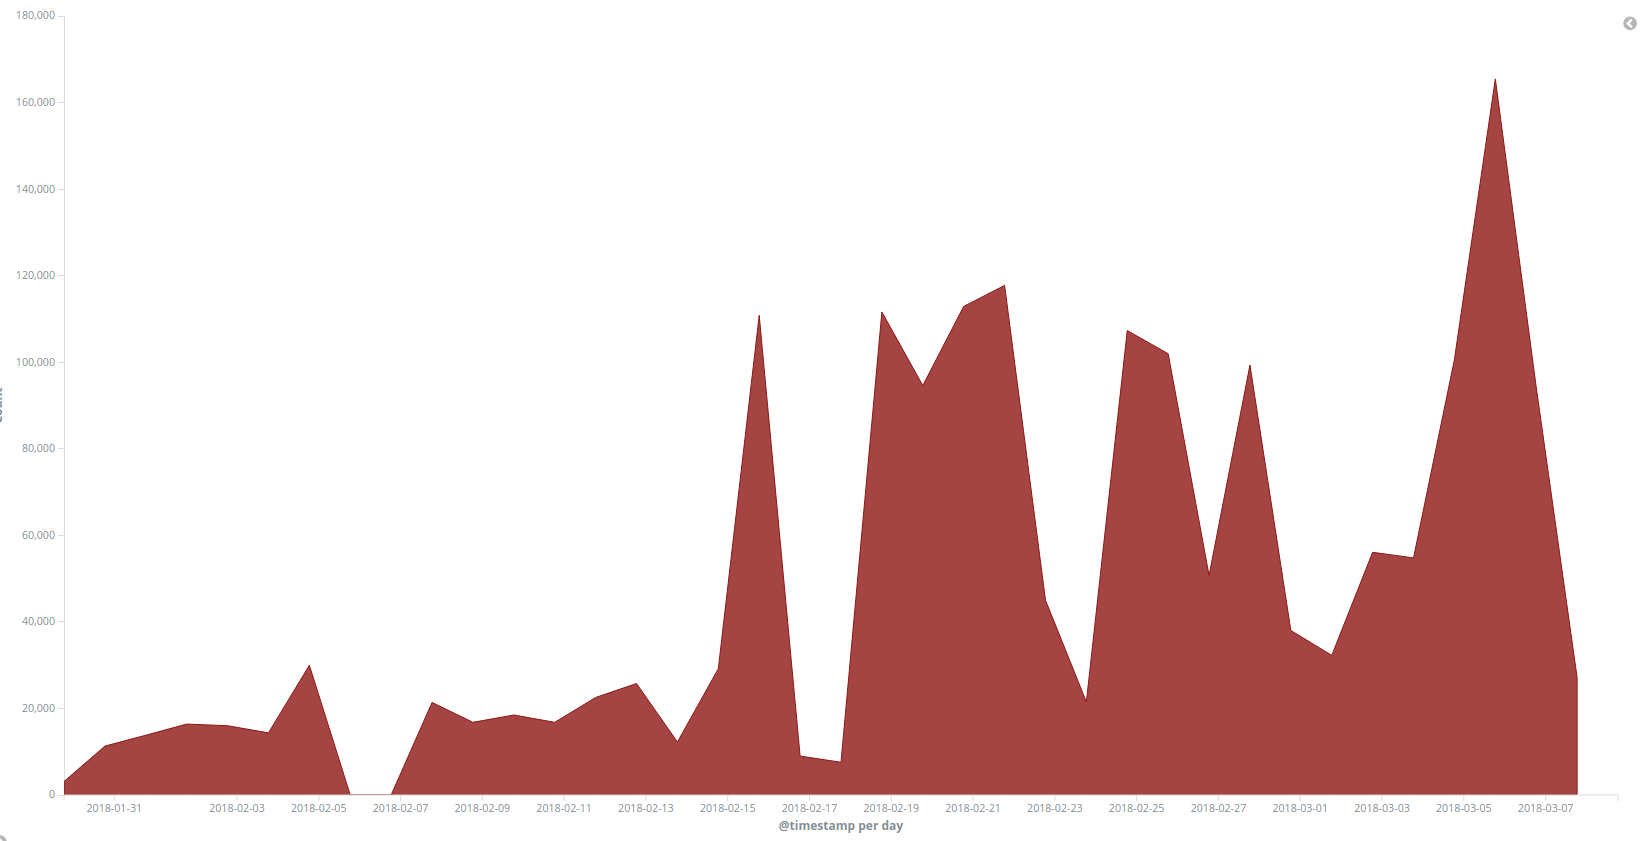
\includegraphics[scale=0.2]{Daily_Attacks_Count}
\end{figure}


\item Top 20 Usernames Histogram
\paragraph{}
A Histogram was used to represent the top 20 usernames that have been used by the attackers and intruders.

\begin{figure}[H]
\centering
\caption{Top 20 Usernames Histogram}
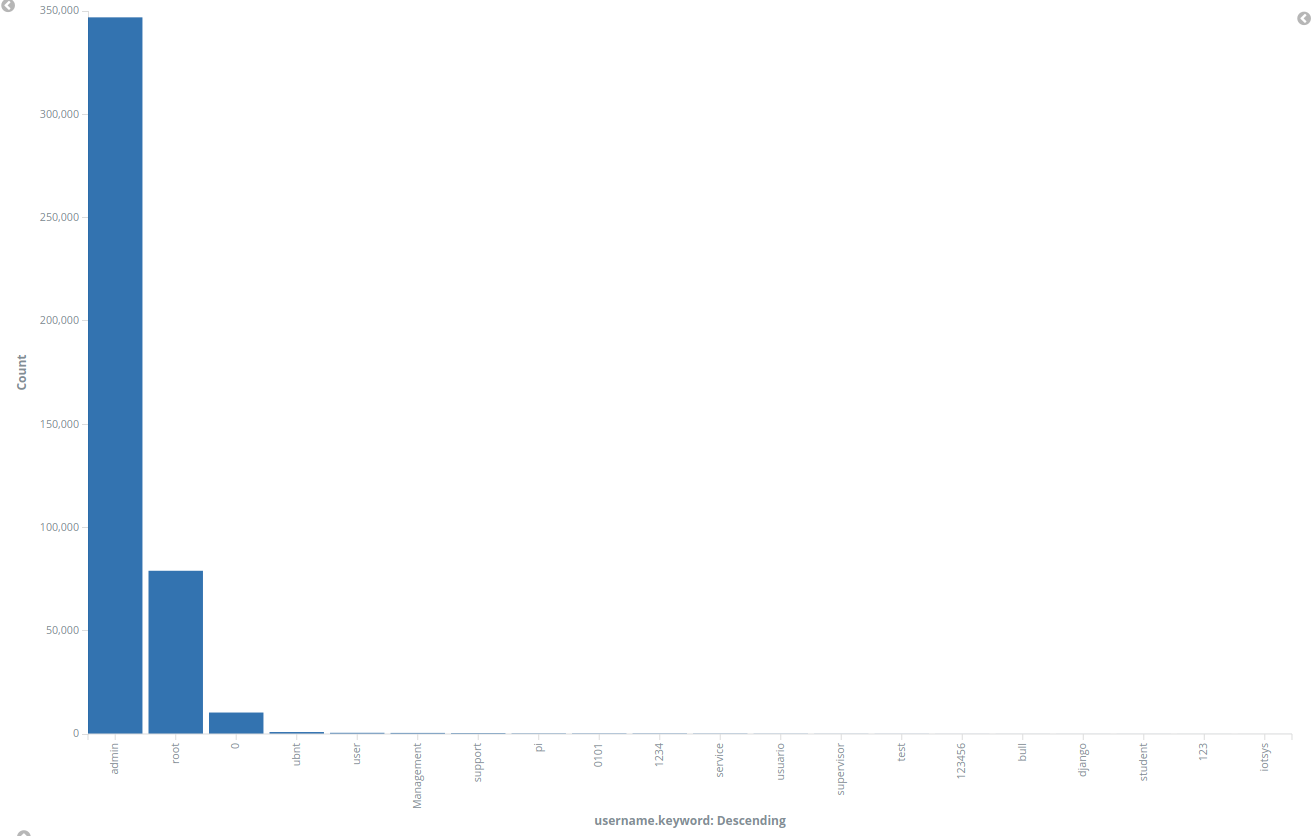
\includegraphics[scale=0.2]{Username_Histogram}
\end{figure}

\paragraph{}
From the graph, it can be observed that username "admin", "root and "ubnt" are mostly used by attackers.

\item Unique Count Of IP's
\paragraph{}
A Kibana Utility graph named Unique Count has been used for counting the Unique Number of IP's till now monitoring system has captured. It has found to be nearly 2000 IP's.

\begin{figure}[H]
\centering
\caption{Unique Count of IP's}

\includegraphics[scale=0.5]{Unique_IP}
\end{figure}

\item Top 20 Passwords Pie
\paragraph{}
A pie chart has been drawn against the top 20 passwords used by the attackers and intruders. It can be observed that passwords "ubnt" and "admin" are mostly used.

\begin{figure}[H]
\centering
\caption{Top 20 Passwords Pie}
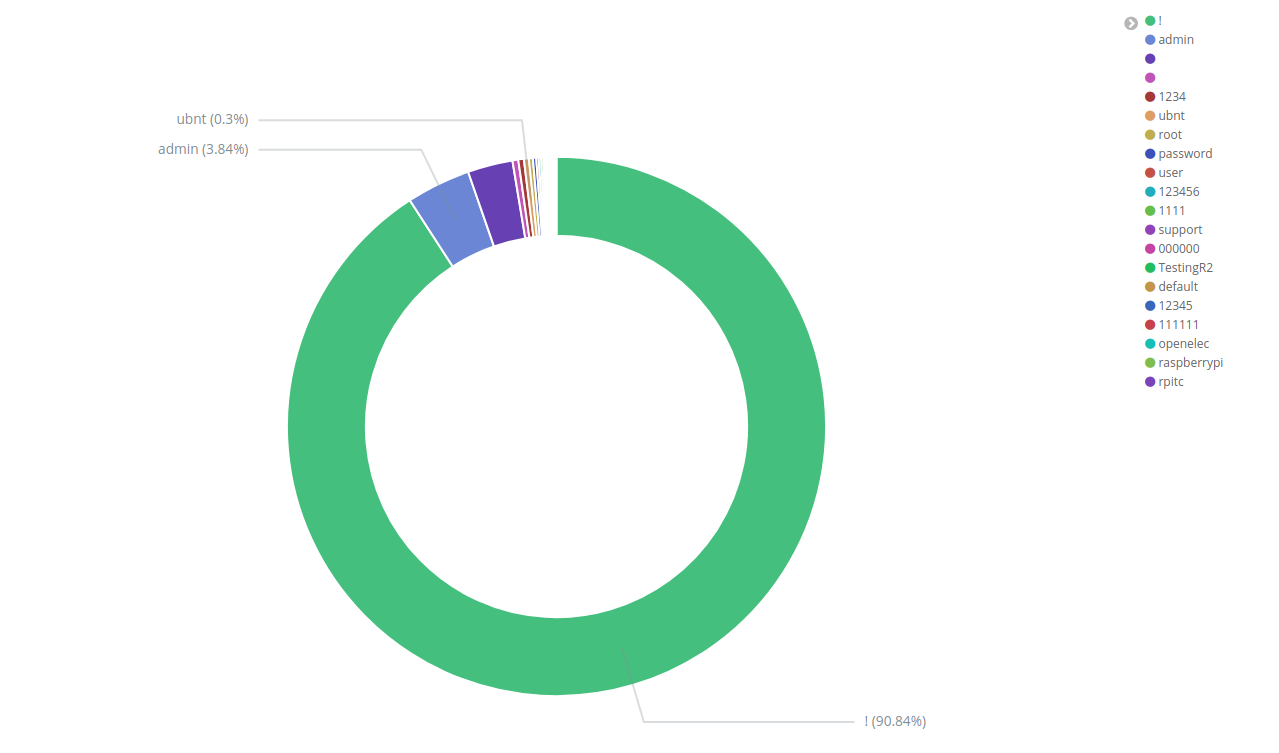
\includegraphics[scale=0.29]{Passwords_Pie}
\end{figure}

\item Global Attacks Map
\paragraph{}
A map is also plotted against the attacks receiving from different contries and continents using the latitude and longitude values. Most of the attacks are received from european continent and china country.

\begin{figure}[H]
\centering
\caption{Global Attacks Map}
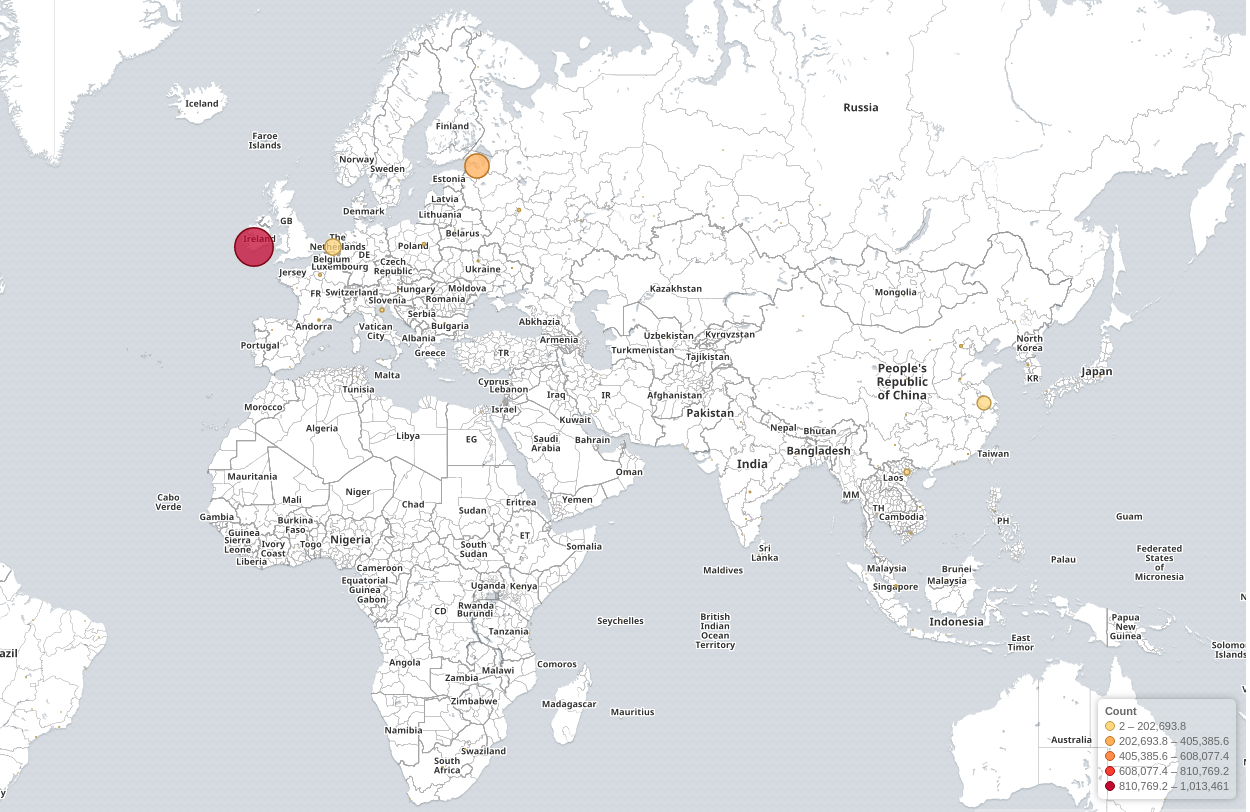
\includegraphics[scale=0.30]{Global_Attacks_Map}
\end{figure}

\end{enumerate}

\subsection{Stochastic Process}
\paragraph{}
Stochastic process is also called random process. It contains random variables with probabilities associated to it. While exact path cannot be inferred, assumptions can be made based on the probabilities of random variables. Attacks pattern observed is following random process or stochastic process as number of attacks on daily basis is not following any pattern.

\begin{figure}[H]
\centering
\caption{Stochastic Process}
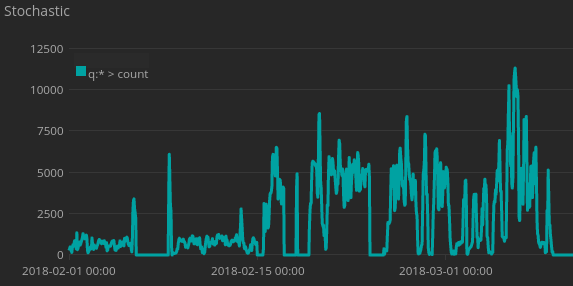
\includegraphics[scale=0.7]{Stochastic_Process}
\end{figure}



































\begin{algorithm}
\caption{Modified Naive Bayes With K-Means Clustering}\label{euclid}
\begin{algorithmic}[1]

\State $\textbf{Probability}\textit{(IP is Malicious / Commands executed by IP }\text{) = }$
\begin{equation*}
  		\frac{\textbf{Probability}\textit{(IP is Malicious) * }\textbf{Probability}\textit{(Commands executed by IP / IP is Malicious)}}{\textbf{Probability}\textit{(Commands executed by IP)}}
	\end{equation*}
\State $\textbf{Note :}\textit{As we are working on Unclassified Data,We are assuming below values.}$
\State $\textbf{Probability}\textit{(IP is Malicious) = }\textbf{1} $
\State $\textbf{Probability}\textit{(Commands executed by IP) = }\textbf{1} $
\State $\textbf{Probability}\textit{(Commands executed by IP / IP is Malicious) = }$

\begin{equation*}
  		\frac{\textit{Frequency of Word + 1 (Smoothening Factor)}}{\textit{ Total Number of Words + Unique Number of Words}}
	\end{equation*}

\State $\textbf{Note :}\textit{ Commands executed by each IP is split into words and their }$
$\centerline{\textit{frequencies are stored in Database}}$
\State $\textit{Total No of Words} \gets \textit{N}$
\State $\textit{Unique No of Words} \gets \textit{dict}$
\While {$\textit{IP List} \textbf{ not } \textit{Empty} $}
	\State $\textit{No of Words} \gets \textit{Splitting Commands into words}$
	\State $\textbf{Probability}\textit{(IP is Malicious / Commands executed by IP }\text{)}$
	\State $\textbf{= Probability (}\textit{Commands executed by IP / IP is Malicious}) $ 
	\State $\textbf{= }\prod_{i=1}^{\textit{No of Words}}\textbf{Probability}\textit{(}\textit{Word}_i\textit{ in Command Executed/ IP is Malicious)}$
	\State $\textbf{= }\prod_{i=1}^{\textit{No of Words}}\frac{\textit{n}_i\textit{+ 1 }}{\textit{ N + dict}}$	
	
\EndWhile
\State $\textbf{done}$
\State $\textbf{Note : }\textit{ Each IP Final Probability will be stored in Database}$

\State $\textbf{Note : }\textit{After Storing the IP's Probabilities in Database,}\textbf{K-Means} $ $\textit{Clustering algorithm is applied to classify the IP's into two classes as high and Low.}$
 $\centerline{***********************************}$
 $\textbf{\centerline{K-Means is given below}}$
 $\centerline{***********************************}$
\State $\textbf{Input : }\textit{Set of Data Points }\textbf{D}\textit{ and No. of Clusters}\textbf{ K.}$
\State $\textbf{Output : }\textit{Cluster Centers that minimizes the squared error distortion.}$
\State $\textbf{Algorithm : }$
\begin{enumerate}
   \item \textit{Pick K Data points randomly from D to form cluster centers.}
   \item \textit{Assign each data point to its nearest cluster center by calculating and taking the minimum Euclidean Squared distance metric.}
   \item \textit{After all data points are assigned to their clusters,move each cluster center to mean of its assigned data points.}
   \item \textit{With new cluster centers, repeat 2 to 3 until there is no convergence.}
\end{enumerate}

\end{algorithmic}
\end{algorithm}


\end{document}
